\graphicspath{{figures/design/}}


\chapter{Test Journal: Servomotors}
\label{ssc:Servomotors}

\begin{table}[!h]
\begin{tabular}{l l}
\textbf{Test participants:} & Romain \& Raphael   \\
\textbf{Date:}  & 01/05-2017
\end{tabular}
\end{table}

\section*{Purpose}
	
The purpose of the test is to verify the proper functioning of the servomotors, and calculate the time constant of the servomotors' required tasks.
	
\section*{Test equipment and components}


\begin{table}[htbp]
	\centering
	\caption{List of measurement equipment and components}\label{tab_appendix:Servo_equip2}
	
	\begin{tabularx}{\textwidth}{lXX}
		Name & Brand	& Model \\ \toprule 
		Servomotors	& SpringRc & SM-s2309s 	\\ \rowcolor{lightGrey}
		Controller	& Arduino & Arduino Nano \\ 
		Camera & Samsung & 0 \\ \rowcolor{lightGrey}
		Media Player Classic & Gabest & Home Cinema\\ 
	\end{tabularx}
\end{table}




	\section*{Setup}
	
The servomotors are controlled and powered by an Arduino Uno. Three different position of the servomotors sticks are set up by code found in the attachements. The measurement setup is seen on the photos of the three different positions. \

\begin{figure} [htbp]
	\centering
	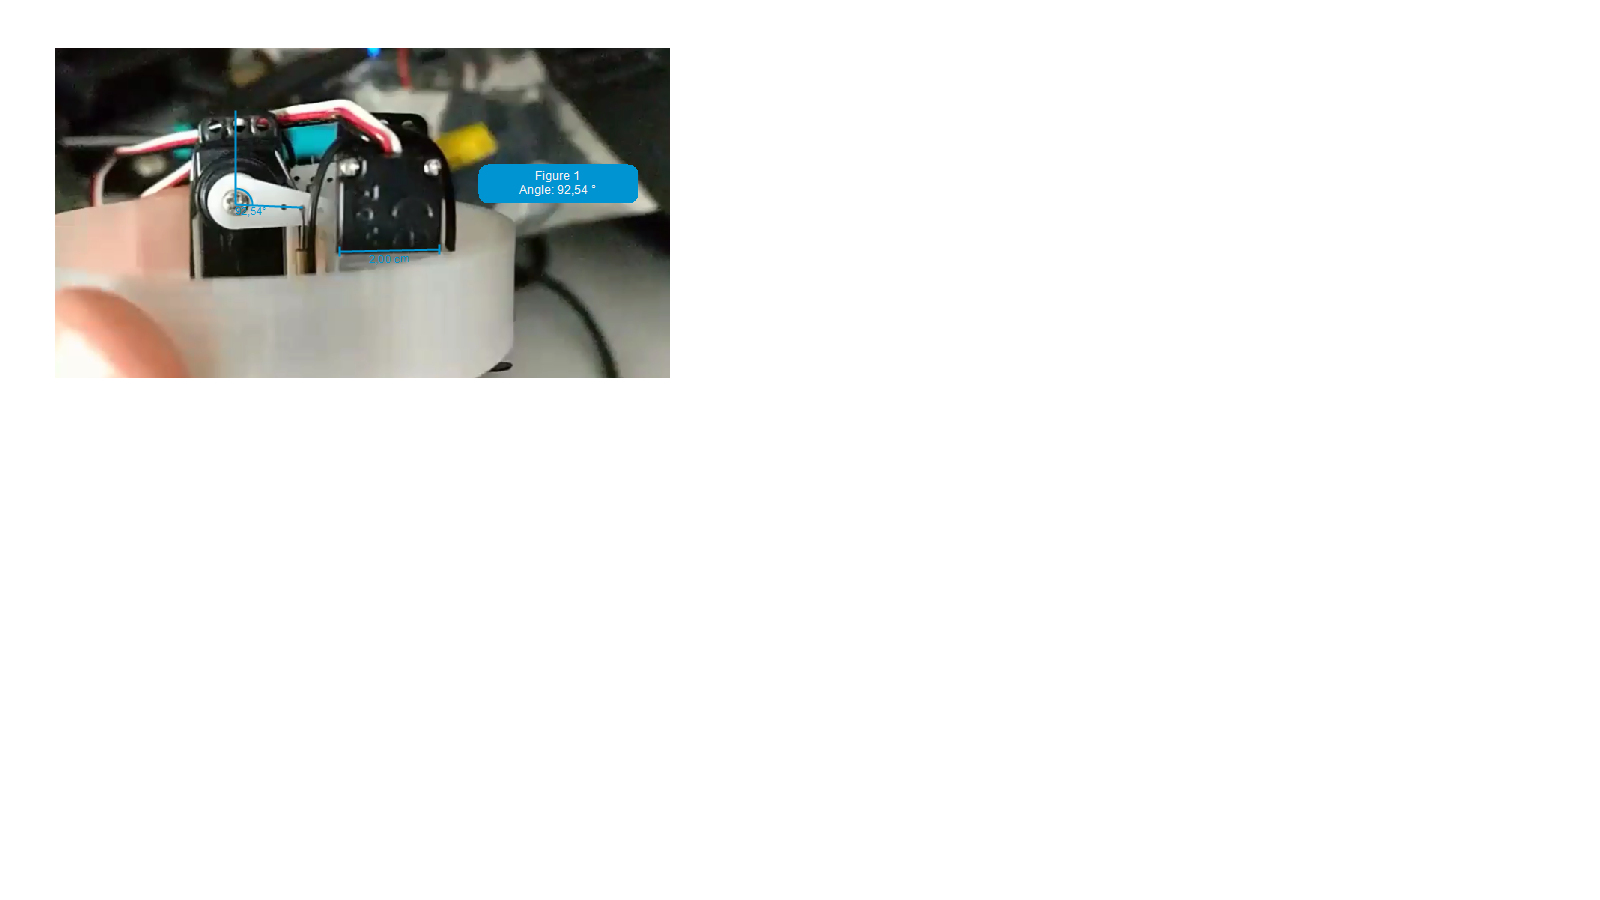
\includegraphics[width=0.50\linewidth]{figures/"Rocket"/"Servomotors"/middlepositionangle.png}
	\caption{Photograph of the servomotor at the medium position.} \label{fig:ServoInitialPosition}
\end{figure}

\begin{figure} [htbp]
	\centering
	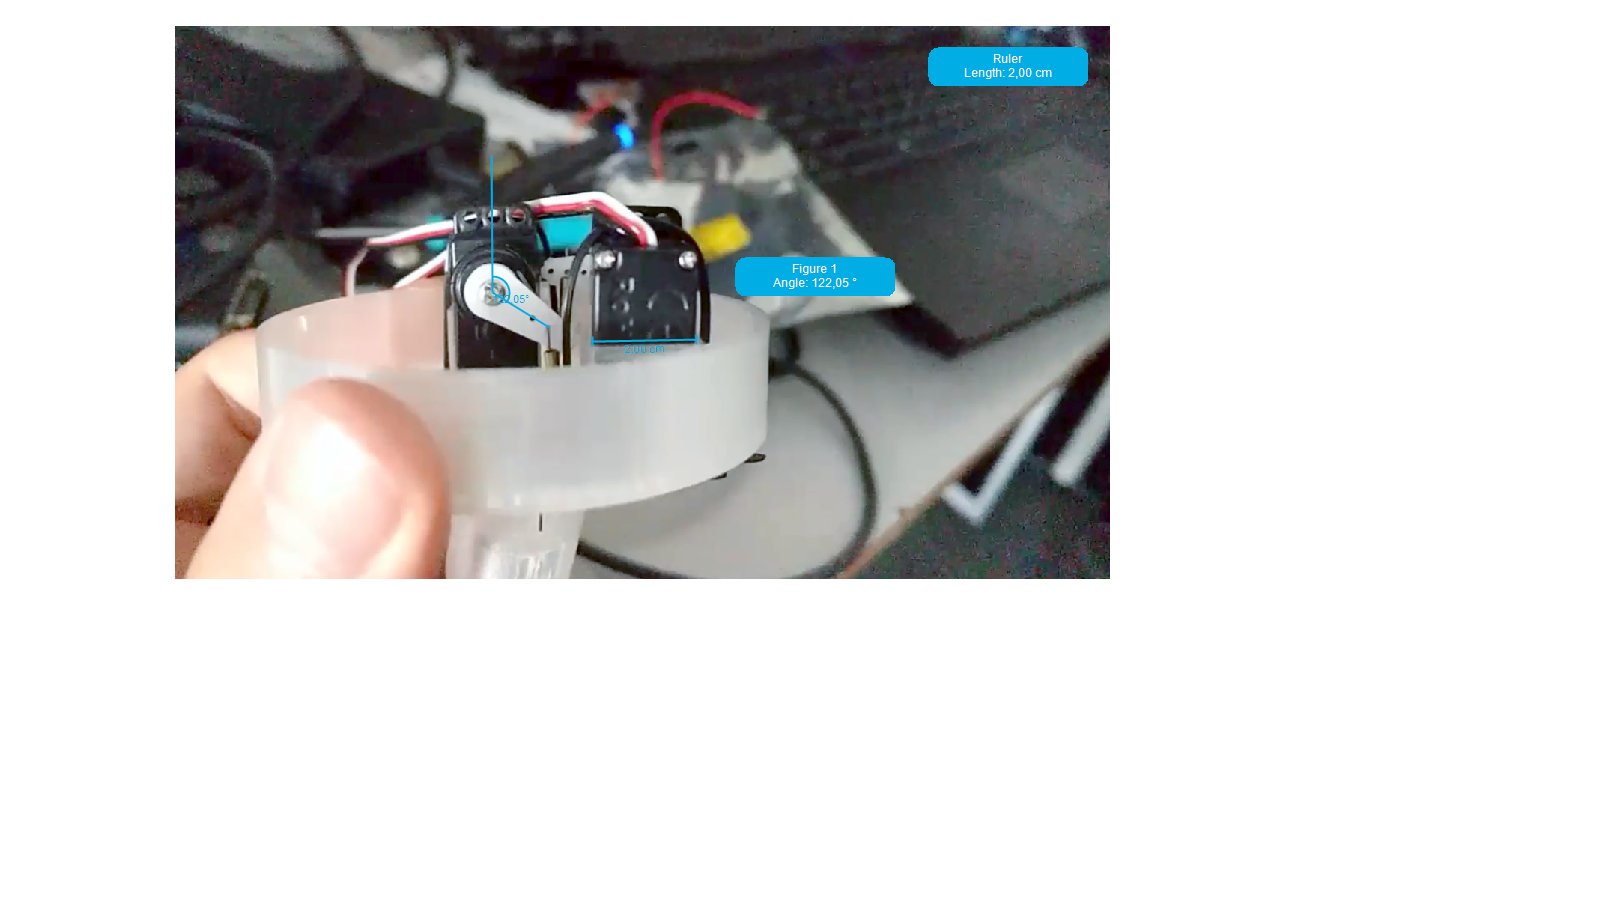
\includegraphics[width=0.50\linewidth]{figures/"Rocket"/"Servomotors"/downpositionangle.png}
	\caption{Photograph of the servomotor at the lower position.} \label{fig:ServoLowPosition}
\end{figure}

\begin{figure} [htbp]
	\centering
	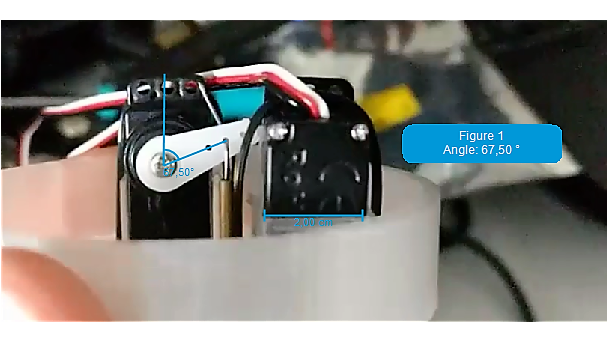
\includegraphics[width=0.50\linewidth]{figures/"Rocket"/"Servomotors"/highpositionangle.png}
	\caption{Photograph of the servomotor at the higher position.} \label{fig:ServoHighPosition}
\end{figure}


	\section*{Method}
	
 The servomotors' arms are controlled to go from one position to another set one. The process is filmed in slow motion in order to analyse it. An x/y basis is used with the base set at the rotation center.
  
		\subsubsection*{Angle variation}
		
The angle variation is found by measuring the angle difference betwwen the horizontal axis and the stick direction. The servomotors function properlly if the angles desired correspond to the real angles.

		\subsubsection*{Time constant}
		
In order to find the time constant, the time to go from one position to another is measured using the video software. The time constant is equal to $63$ per cent of the total time from one position to another. 



	\section*{Raw data}
	
		\subsubsection*{Angle variation}


\begin{table}[htbp]
	\centering
	\caption{Measurement time of different set points.}
	\label{tab:AngleData}
	\begin{tabularx}{\textwidth}{lX} 
		Position & Angle{(}°{)}  \\ \toprule
		Lowest & $122.05$  \\ \rowcolor{lightGrey}
		Middle & $92.54$  \\ 
		Highest & $67.50$  \\
	\end{tabularx}
\end{table}
		
		
		
	
		\subsubsection*{Time constant}

\begin{table}[htbp]
	\centering
	\caption{Measurment time of different set points.}
	\label{tab:TimeData}
	\begin{tabularx}{\textwidth}{lXXX} 
		Test & Time of departure {(}s{)}& Time of arrival{(}s{)} & total time {(}s{)} \\  \toprule 
		$1$     & $2.507$              & $2.641$             & $0.134$                     \\   \rowcolor{lightGrey}
		$2$     & $2.508$              & $2.642$ & $0.134$                                 \\
		$3$     & $60.066$              & $61.133$ & $0.133$                                 \\ \rowcolor{lightGrey}
		$4$     & $60.033$             & $61.082$            & $0.131$                    \\ 
	\end{tabularx}
\end{table}
				
%%				test table
%\begin{table}[htbp]
%	\begin{tabular}{|l||c|c|} \hline\hline
%		Ice Cream Store & Location & How to Get There \\ \hline
%		Toscanini’s & Central Square & Just walk! \\
%		Herrell’s & Harvard Square & Red Line \\
%		J.P. Licks & Davis Square & Red Line \\
%		Ben \& Jerry’s & Newbury Street & Green Line \\ \hline\hline
%	\end{tabular}
%\end{table}

	\section*{Data processing}	
	
		\subsubsection*{Angle variation}
		
The angle variation is found by measuring the angle difference betwwen the horizontal axis and the stick direction. The desired angle difference between the different positon is $30$ \si{\degree}. The servomotors function properlly if the angles desired correspond to the measured angles.

\begin{subequations}
	\begin{flalign}
		& a_{mh} = 29.51 \si{\degree} \\  
		& a_{ml} = 25.04 \si{\degree}
	\end{flalign}
\end{subequations}
\startexplain
\explain{$a_{mh}$ is the angle difference between the middle to highest position of the servomotor's arm}{\si{\degree}}
\explain{$a_{ml}$ is the angle difference between the middle to lowest position of the servomotor's arm}{\si{\degree}}
\stopexplain

The error comes from measure errors and to the servomotors lifting a weight.

		\subsubsection*{Time constant}
		
 In order to find the time constant, the time to go from one position to another is measured using the video software. The time constant is equal to $63$ per cent of the mean value of the total time from one position to another : 
 \begin{subequations}
 	\begin{flalign}
 		& t_{constant} = \frac{63}{100} \cdot t_{mean} \\
 		& t_{constant} = \frac{63}{100} \cdot 0.133 = 0.084
 		\label{eq:TfC1C2}
 	\end{flalign}
 \end{subequations}
 \startexplain
\explain{$ t_{constant}$ is the motor input voltage}{\si{\second}}
\explain{$t_{mean}$ is the mean value of the total time from one position to another}{\si{\second}}
\stopexplain
 
 

	\section*{Conclusion}
	
The image analysis presents errors. The range of required angle movement of the servomotors is inferior to $30$ degrees, meaning that the servomotors are considered as meeting the requirements even thought errors are present. The time constant of the servomotors is $0.084$ and meets the requirement of a fast reaction to a controller command.





